\documentclass{beamer} 
\usepackage{amsmath,amsthm}
\usepackage{graphicx,microtype,parskip}
\usepackage{caption,subcaption,multirow}
\usepackage{attrib}

\frenchspacing

\usetheme{default}
\usecolortheme{whale}

\setbeamertemplate{navigation symbols}{}

\setbeamercolor{title}{fg=blue,bg=white}

\setbeamercolor{block title}{fg=white,bg=gray}
\setbeamercolor{block body}{fg=black,bg=lightgray}

\setbeamercolor{block title alerted}{fg=white,bg=darkgray}
\setbeamercolor{block body alerted}{fg=black,bg=lightgray}

\title{Death and taxa}
\subtitle{time-invariant differences in mammal species duration}
\author{Peter D Smits}
\institute{Committee on Evolutionary Biology}
\titlegraphic{
  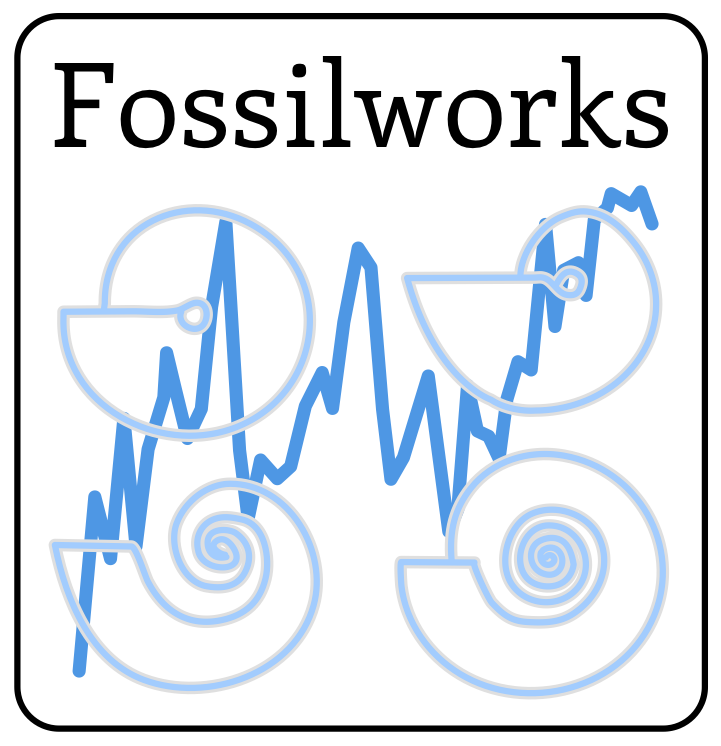
\includegraphics[width=1.75cm,height=1.75cm,keepaspectratio=true]{figure/fossilworks}
  
\includegraphics[width=2.5cm,height=2.5cm,keepaspectratio=true]{figure/paleodb}
  \hspace*{0.35\paperwidth}
  
\includegraphics[width=1.75cm,height=1.75cm,keepaspectratio=true]{figure/chicago}
}
\date{}

\begin{document}

\begin{frame}
  \titlepage
\end{frame}

\begin{frame}
  \frametitle{Differences in species duration}

  \begin{block}{Framework}
    \begin{itemize}
      \item How do different species-level ecological traits relate to differences in species duration?
      \item How do time of origination and phylogenetic history contribute to differences in species duration?
      \item Does extinction risk vary with species duration?
      \item Is the current biodiversity crisis consistent with intensification of background or sometimes else (e.g. mass extinction)?
    \end{itemize}
  \end{block}
\end{frame}

\begin{frame}
  \frametitle{System and traits of interest}

  \begin{columns}
    \begin{column}{0.5\textwidth}
      \begin{itemize}
        \item Mammal species
          \begin{itemize}
            \item \(\sim\) 2000
          \end{itemize}
        \item North America
        \item Cenozoic
          \begin{itemize}
            \item \(\sim\) 65 My
          \end{itemize}
        \item duration in 2 My bins
        \item georeferenced occurrences
      \end{itemize}
    \end{column}
    \begin{column}{0.5\textwidth}
      \begin{itemize}
        \item Covariates of interest
          \begin{itemize}
            \item bioprovince occupancy
            \item body size
            \item dietary category: carnivore, herbivore, insectivore, omnivore
            \item locomotor category: arboreal, ground dwelling, scansorial
          \end{itemize}
        \item Structure
          \begin{itemize}
            \item origination cohort
            \item phylogenetic position
          \end{itemize}
      \end{itemize}
    \end{column}
  \end{columns}
\end{frame}

%\begin{frame}
%  \frametitle{Bioprovince occupancy}
%  raster globe, assign occurrance
%  create bipartite graph, map equation to estimate bioprovinces
%\end{frame}

\begin{frame}
  \frametitle{Body size}

  \begin{block}{Hypotheses}
    \begin{itemize}
      \item increase body size, decrease reproductive rate, increase extinction risk.
      \item increase body size, increase geographic range, decrease extinction risk.
      \item no effect.
    \end{itemize}
  \end{block}
\end{frame}

\begin{frame}
  \frametitle{Dietary category}

  carnivory, herbivory, insectivory, omnivory
\end{frame}

\begin{frame}
  \frametitle{Locomotor category}

  arboreal, ground dwelling, scansorial
\end{frame}


\begin{frame}
  \frametitle{Bayesian survival model}
  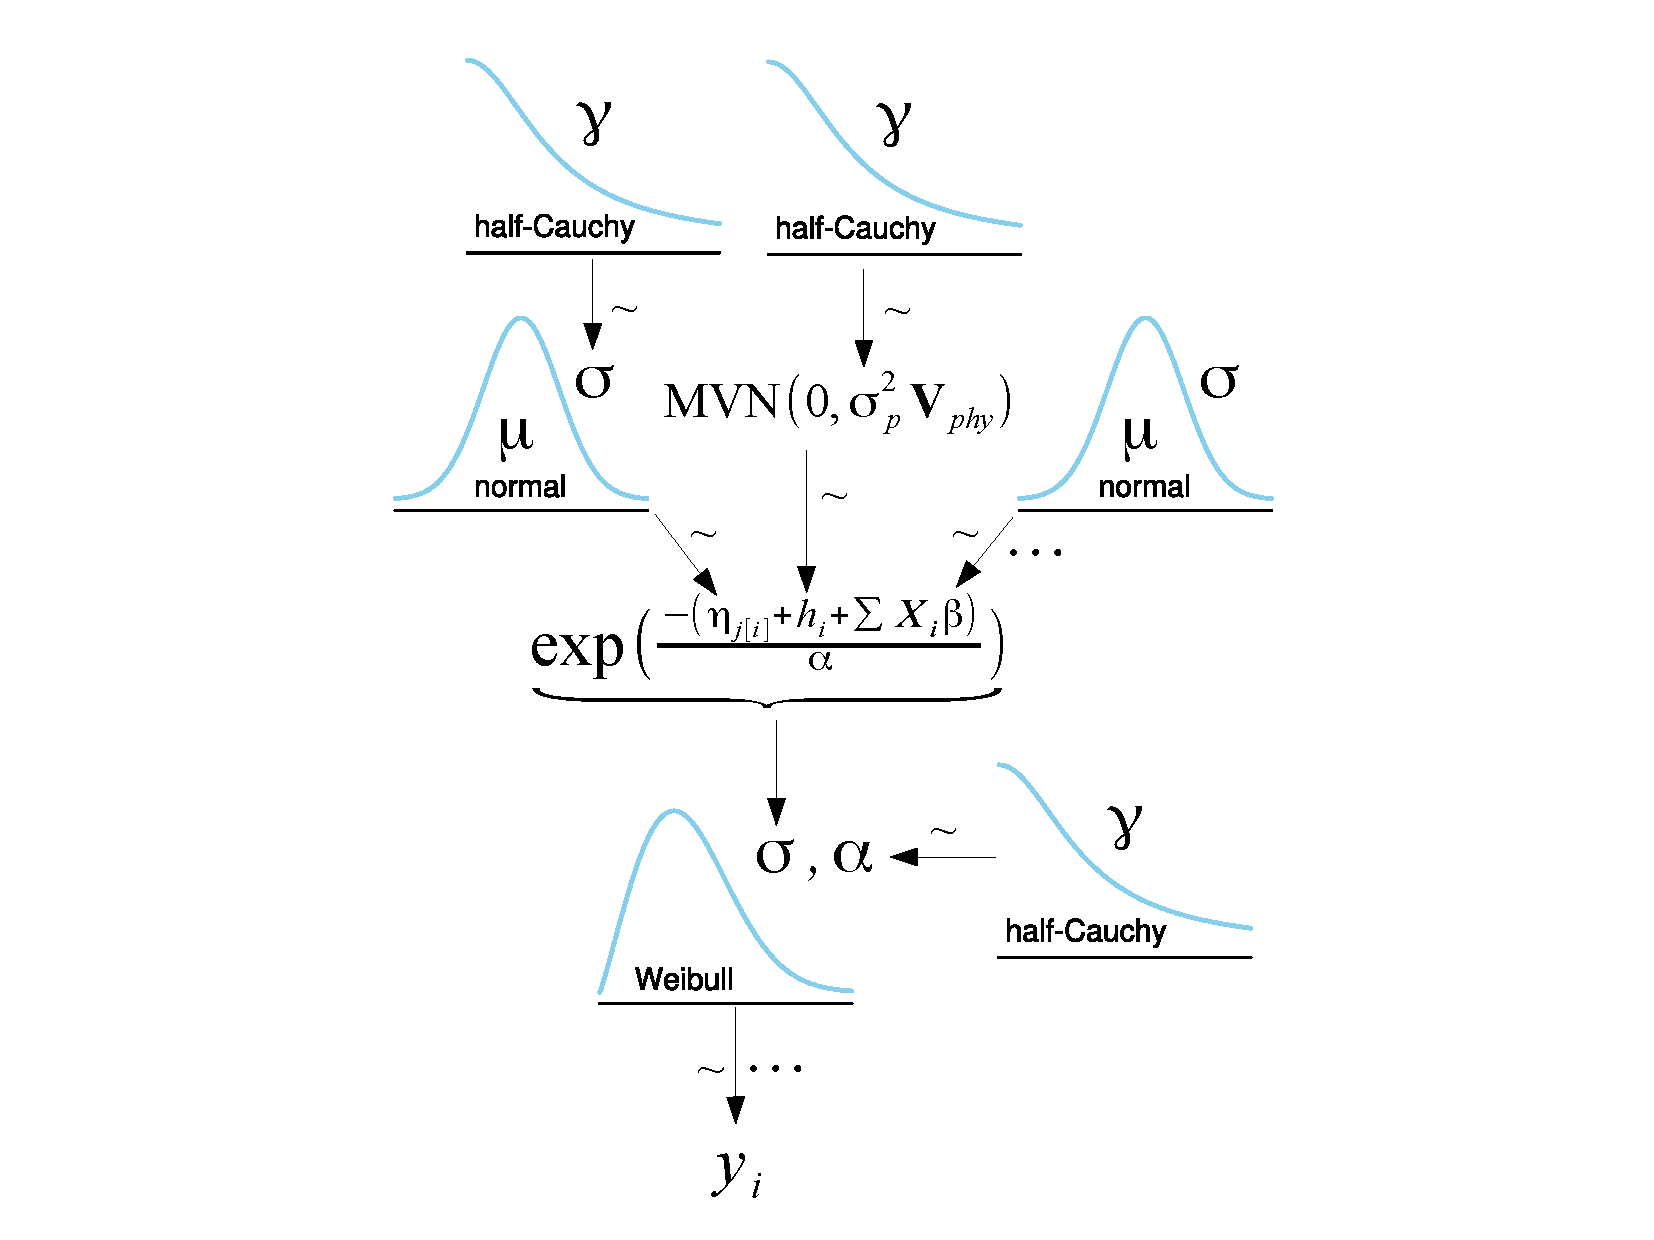
\includegraphics[width=\textwidth,height=0.8\textheight,keepaspectratio=true]{figure/mammal_survival_model}
\end{frame}

\begin{frame}
  \frametitle{Survival function}
\end{frame}

\begin{frame}
  \frametitle{Covariate effects}
\end{frame}

\begin{frame}
  \frametitle{Origination cohort effect}
\end{frame}

\begin{frame}
  \frametitle{Variance partitioning coefficients}
\end{frame}

\begin{frame}
  \frametitle{Current biodiversity crisis}
\end{frame}

\begin{frame}
  \frametitle{Concerns}
\end{frame}

\begin{frame}
  \frametitle{Conclusions}
\end{frame}

\appendix

\begin{frame}
  % blank so i don't just keep going
\end{frame}

\begin{frame}
  \frametitle{Posterior predictive checks: deviance residuals}
\end{frame}

\begin{frame}
  \frametitle{Posterior predictive checks: point check}
\end{frame}

\end{document}
